\section{Make-a-Video}
\label{sec:make_a_video}

Make-a-Video \cite{make_a_video} (2022) by Meta AI is a text-to-video model. Similar to Video-LDM, Make-a-Video extends the text-to-image (T2I) knowledge to diffusion-based text-to-video (T2V) model through spatiotemporally factorized diffusion model. In addition, it doesn't require pairs of text-video data, which allows unsupervised video training, which in turn allows to scale to larger quantities of video data.

They present super-resolution strategies in space and time to generate higher spatial-resolution and higher frame rate video clips, provided a text prompt. They \textbf{leverage image priors} due to the complexity of modeling videos, which simplifies the learning process.







\subsection{Architecture}

\begin{figure}
    \centering
    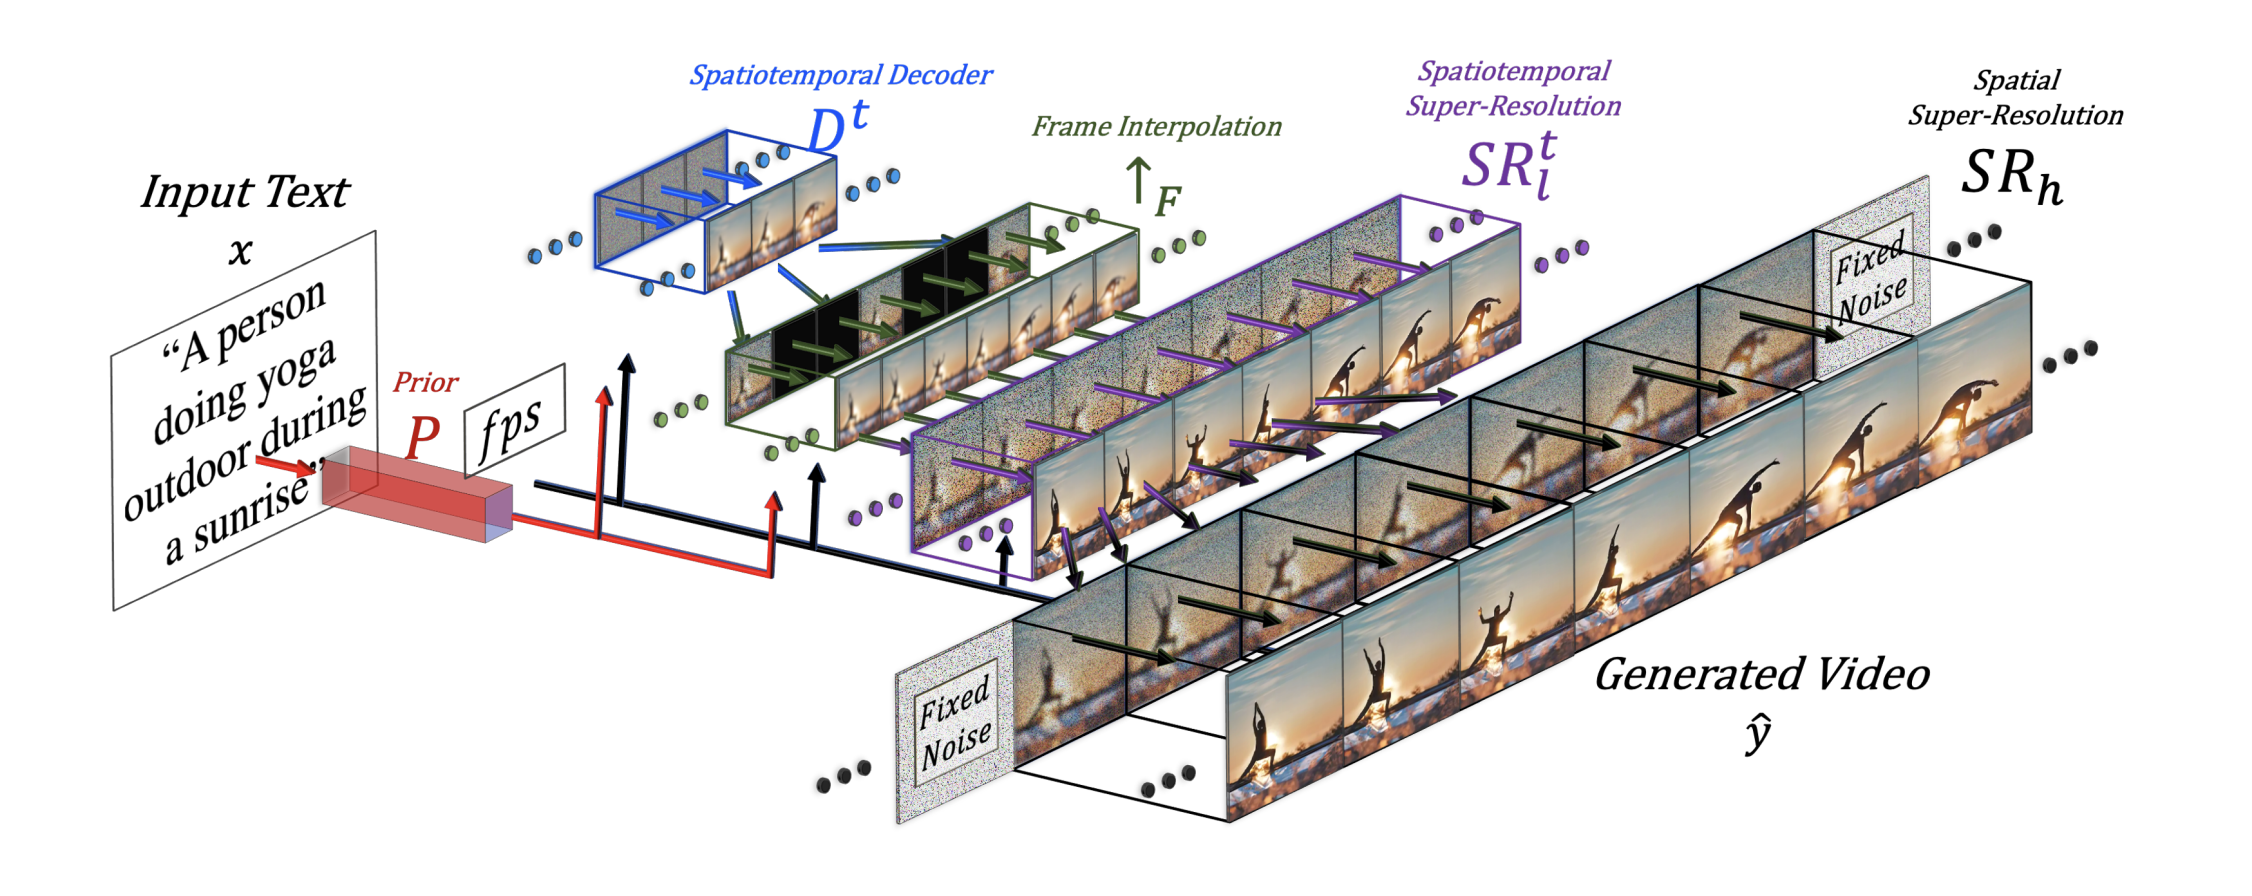
\includegraphics[width=1\textwidth]{images/make_a_video/overview.png}
    \caption{Make-a-Video model high-level architecture overview.}
    \label{fig:make_a_video_overview}
\end{figure}

In figure \ref{fig:make_a_video_overview}, given a text input $x$, its translated into the image embedding prior $P$. The model input is "fps" (frames per second). The \textbf{spatio-temporal decoder $\textcolor{blue}{D^t}$} generates 16 $64\times 64$ frames, which are interpolated into higher fps by the \textbf{frame interpolation model $\textcolor{OliveGreen}{\uparrow_F}$}. Then these frames are increased in spatial resolution to $256\times 256$ by the \textbf{spatiotemporal super-resolution model $\textcolor{Plum}{SR_l^t}$}; and finally increased to resolution $768\times 768$ by \textbf{spatial super-resolution model $SR_h$}. The final output is high-spatiotemporal-resolution video $\hat{y}$.

As discussed above, Make-a-Video has three main components:

\begin{itemize}
    \item Text-to-image model trained on text-image pairs, which is based on the previous work of the OpenAI paper DALL-E 2 \cite{dalle_2} (section \ref{sec:dalle_2}).
    \item Spatiotemporal convolution and attention layers.
    \item Frame interpolation network $\textcolor{OliveGreen}{\uparrow_F}$.
\end{itemize}

The formal mathematical formulation of the Make-a-Video inference is as follows:

\[ \hat{y_t} = \text{SR}_h \circ \textcolor{Plum}{\text{SR}_l^t} \circ \textcolor{OliveGreen}{\uparrow_F} \circ \textcolor{blue}{D^t} \circ \textcolor{Maroon}{P} \circ \left( \hat{x}, C_x (x) \right) \]

where $\mathbf{C_x}$ is the \textbf{CLIP text encoder} and $x$ is the input text.







\subsection{The T2I model}

The T2I model is based on the core components of the OpenAI paper \cite{dalle_2}. In this paper, OpenAI created a model that is called unCLIP (commonly known as DALL-E 2). See section \ref{sec:dalle_2} for more details. They first trained the T2I model, and only then they apply factorization on the T2I model to create the T2V model. We will discuss this T2I model here and explain how they transfer this spatial knowledge to video later.

In Make-a-Video the \textcolor{Maroon}{prior network $P$} generates CLIP image embeddings $y_e$ given CLIP text embeddings $x_e$ (using CLIP text encoder the text prompt is converted to $y_e$).

Then these image embeddings $y_e$ are used to condition the \textcolor{blue}{diffusion based decoder $D$} that generates a single $64\times 64$ image $\hat{y_l}$.

Then two super-resolution networks $\textcolor{Plum}{\text{SR}_l}$ and $\text{SR}_h$ are applied to increase the resolution to $256\times 256$ and $768\times 768$ respectively to generate the final image $\hat{y}$.

The researchers note that they then downsample the image to $512\times 512$ using bicubic interpolation for cleaner aesthetics.







\subsubsection{DALL-E 2}
\label{sec:dalle_2}

DALL-E 2 is a text-to-image model, which leverages contrastive models like CLIP for image generation. They proposed a two-stage model: 

\begin{itemize}
    \item a prior network $P(z_i | y)$ that generates CLIP image embeddings $z_i$ conditioned on captions
    \item and a diffusion based decoder $P(x | z_i, y)$ that generates images $x$ conditioned on these image embeddings $z_i$, and optionally the captions $y$.
\end{itemize}

\begin{figure}
    \centering
    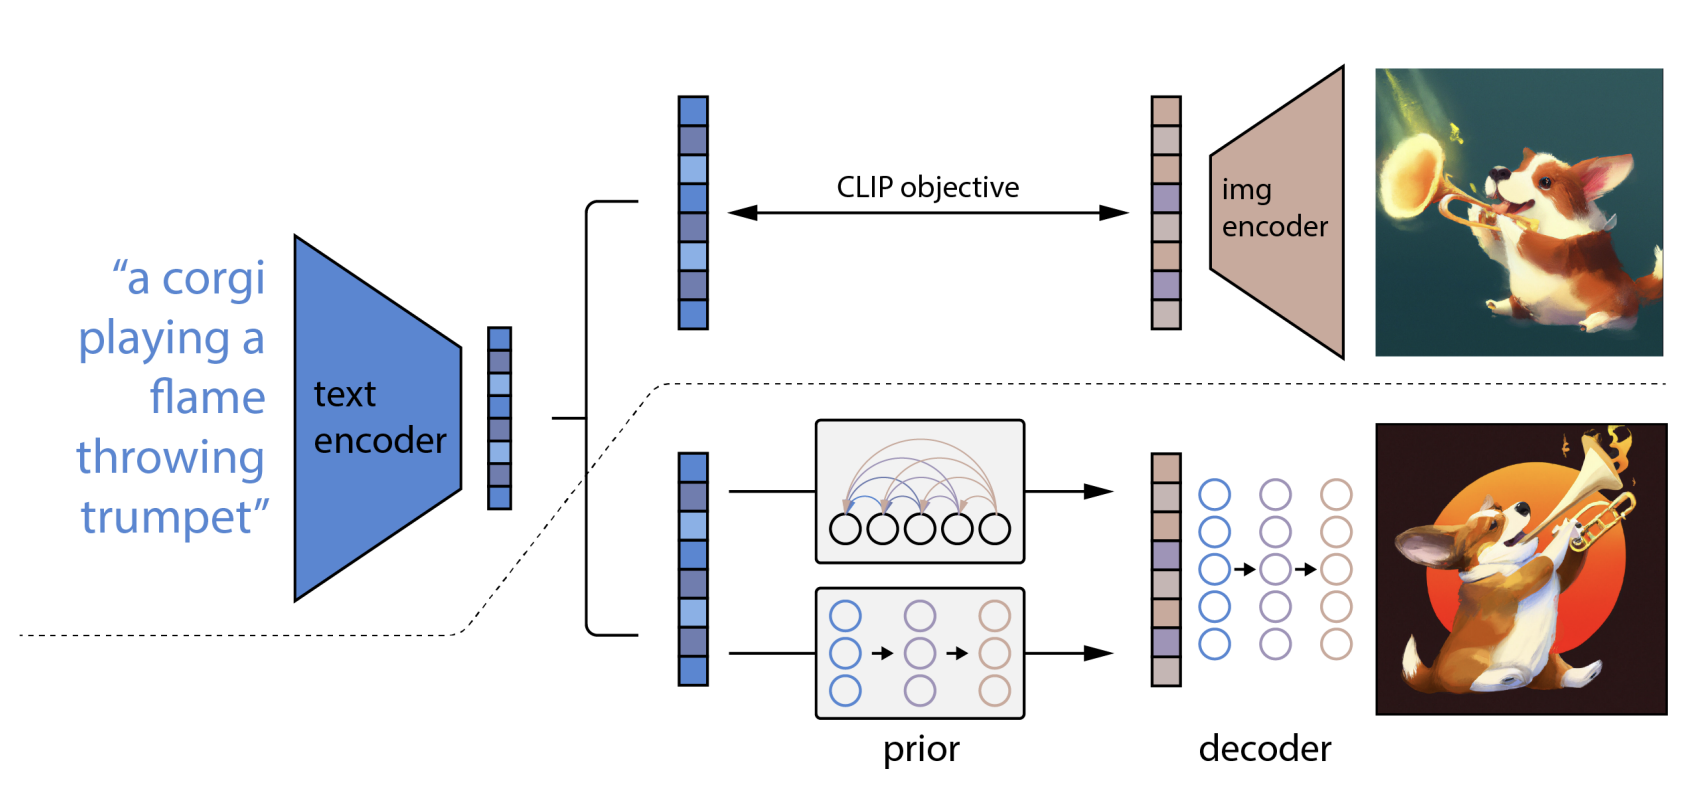
\includegraphics[width=0.7\textwidth]{images/make_a_video/dalle_2.png}
    \caption{High level overview of unCLIP (DALL-E 2) \cite{dalle_2} by OpenAI. The top figure shows the training objective of DALL-E 2, and the bottom figure shows the inference process. The prior model takes the CLIP text embeddings $z_t$ and generates image embeddings $z_i$. Then the decoder takes in image embeddings $z_i$ and generates the final image.}
    \label{fig:make_a_video_dalle2_overview}
\end{figure}

In figure \ref{fig:make_a_video_overview}, we can see the training objective of DALL-E 2 and the inference process. The decoder acts as inverted CLIP encoder. Given inputs $(x, y)$ where $x$ are images and $y$ are their caption, then $z_i$ is the corresponding CLIP image embeddings and $z_t$ is the CLIP text embeddings.

They tested which prior network works the best: autoregressive (with a transformer to autoregressively predict the image embeddings, conditioned on the text captions and CLIP text embeddings by encoding them as prefix to the sequence) or diffusion based prior network, and they went with diffusion. 

The diffusion based prior network is based on decoder-only transformer architecture and trained it on a sequence consisting of the encoded text, the CLIP text embedding, the diffusion timestep, and the noised CLIP image embedding. The reason that the diffusion network uses transformer is because of the nature of the input-output: the input and output are sequence, and they aren't using U-Net but a decoder-only transformer for this downstream task.

The researchers used a diffusion model in the decoder to process images conditioned on CLIP image embeddings (and optionally text captions). The condition mechanism is similar to how the time-step embeddings are injected into Stable Diffusion.







\subsection{Expanding the T2I model to video domain}

The researchers modify the T2I model and transfer the image knowledge to video domain by expanding the 2D conditional network into the temporal dimension.

In short, they added support of the temporal dimension in the convolutional layers and attention layers. The fully-connected layers doesn't need factorization since they are agnostic to structured spatial and temporal information.

\subsubsection{Spatiotemporal layers}

The main modifications that were made to the T2I model was in the diffusion based U-Net backbone. The spatiotemporal decoder $\textcolor{blue}{D^t}$ now \textbf{generates 16 RGB frames} of $64\times 64$ resolution, instead of one frame.

% TODO: Explain how the interpolation network works
They added a new network: frame interpolation network $\textcolor{OliveGreen}{\uparrow_F}$ which increases the fps by interpolating on the 16 frames from the spatiotemporal decoder (as seen in figure \ref{fig:make_a_video_overview}).

They also modified the spatial layers of the super-resolution network $\text{SR}_l$ to spatiotemporal super-resolution network $\textcolor{red}{\mathbf{\text{SR}_l^t}}$. The reason they chose not operate on the higher-resolution super-resolution network $\text{SR}_h$ because of memory and compute constraints, so the high super-resolution model doesn't work on the temporal dimension, whereas the low super-resolution model $\text{SR}_l$ does (its transformed to $\text{SR}_l^t$).



\subsubsection{Pseudo-3D convolutional layers}

Because 3D convolutional layers are very compute and memory expensive, the researchers opt to go with pseudo 3D convolutional layers.

In \cite{chollet2017xception}, the authors proposed a method to replace 3D convolutions with pseudo-3D convolutions. In this method they decouple the processing of spatial and temporal dimensions, which they call "depthwise separable convolution layers". In Make-a-Video they say that in addition to the more compute efficient convolutions they also want to retain the previously learned spatial knowledge of the T2I model.

First they apply the 2D convolution on spatial axis and only then they apply 1D convolution on the temporal axis. This facilitates information sharing between the spatial and temporal axes.

The pseudo-3D convolutional layer is defined as:

\[ 
\text{Conv}_{\text{P3D}} (h) := \text{Conv}_{\text{1D}} (
    \text{Conv}_{\text{2D}} (h) \circ T
) \circ T \]

where $h \in \mathbb{R}^{B\times C\times F\times H\times W}$ is an input tensor, where $B,\ C,\ F,\ H,\ W$ are the batch, channels, frames, height and width respectively, and $\circ T$ is the transpose operator which swaps between spatial and temporal dimensions.

\begin{figure}
    \centering
    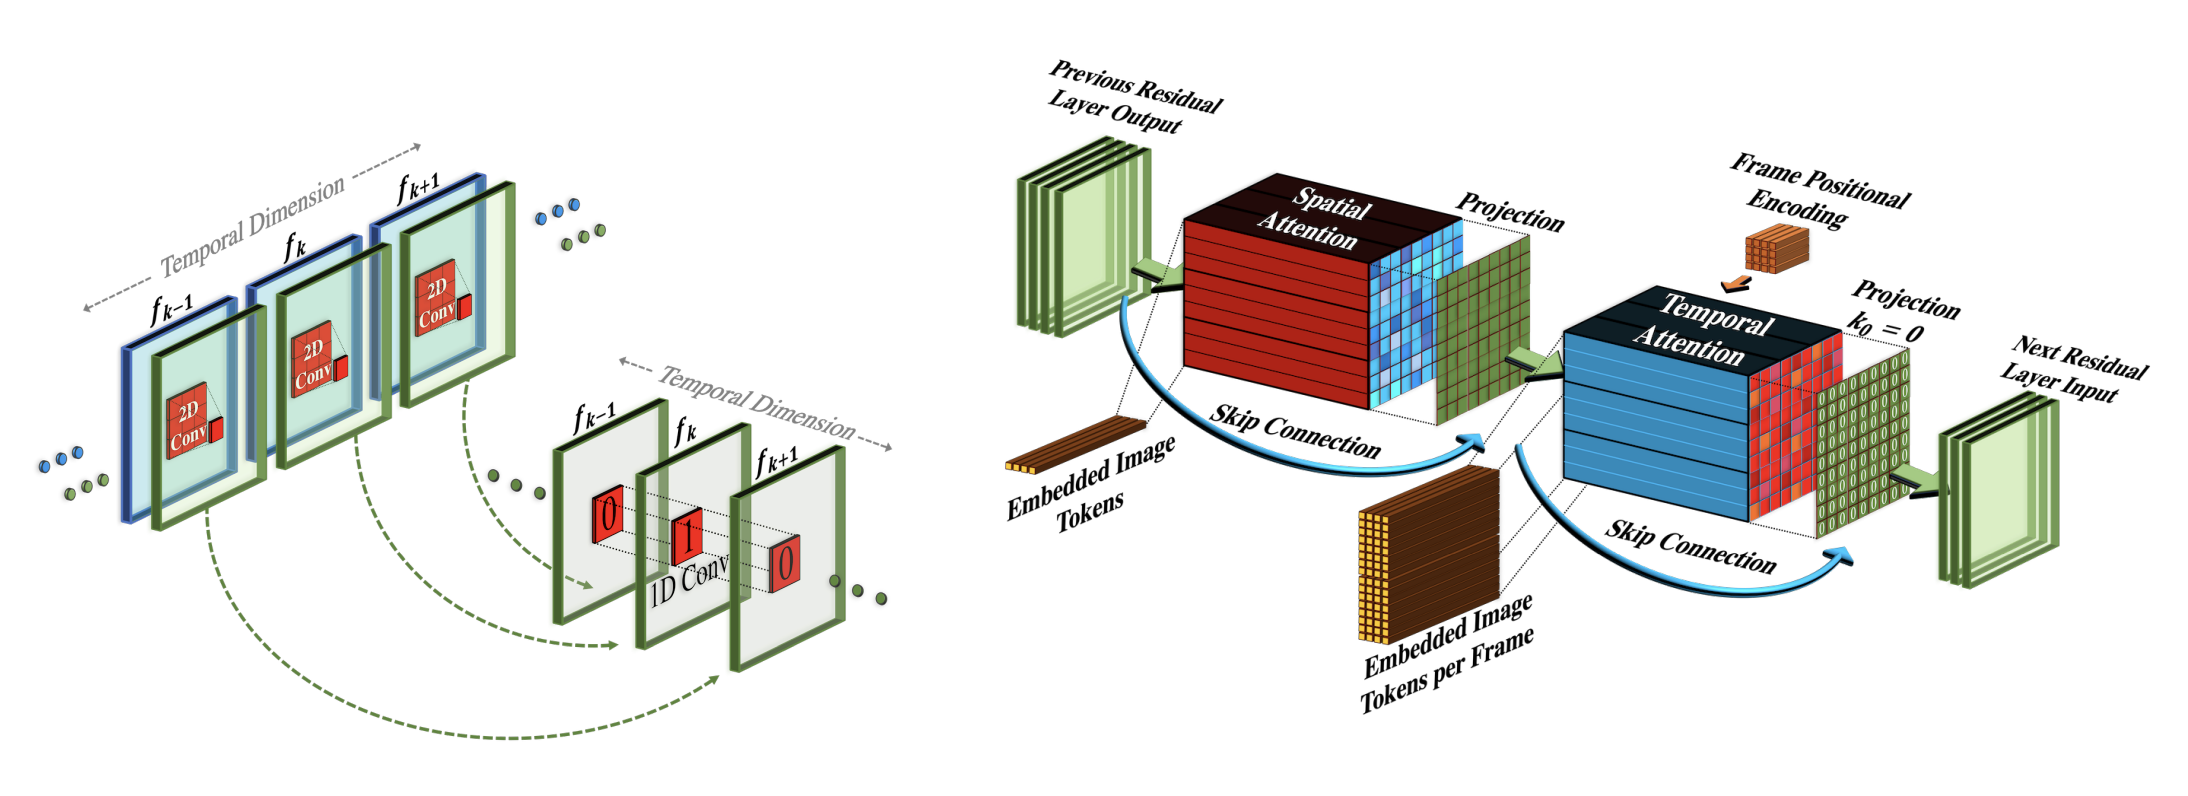
\includegraphics[width=0.7\textwidth]{images/make_a_video/pseudo_3d.png}
    \caption{Architecture of pseudo-3D convolutional and attention layers. Left: Pseudo-3D convolution and initialization. Right: Pseudo-3D attention and initialization.}
    \label{fig:make_a_video_pseudo_3d_conv_and_attention}
\end{figure}

\textbf{Spatiotemporal initialization}: In figure \ref{fig:make_a_video_pseudo_3d_conv_and_attention} we can see the pseudo-3D convolutional layer initialization. After applying 2D spatial convolutions they apply 1D temporal convolution. \textbf{The temporal 1D convolution layer is initialized as the identity function, it performs no transformation on the input data initially}. This way the network relies on the already learned spatial features. \textbf{The temporal consistency will be learned at a later stage}, where the model is trained on video dataset.






\subsubsection{Pseudo-3D attention layers}

Adding the temporal dimension to the attention layers is computationally infeasible. They follow the work of \cite{video_diffusion_models} (Video U-Net).

After each pre-trained spatial attention layer they stack a pseudo-3D temporal attention layer. 

Given tensor a tensor $h$ the \texttt{flatten} operation flattens the spatial dimension to: 

\[ 
h' \in \mathbb{R}^{B\times C\times F\times \mathbf{\textcolor{red}{HW}}} 
\] 

and \texttt{unflatten} operation is the inverse operation. The pseudo-3D attention layer is defined as:

\[ \text{ATTN}_{\text{P3D}} (h) = \text{unflatten} 
(\text{ATTN}_{\text{1D}} 
(\text{ATTN}_{\text{2D}} 
(\text{flatten} (h)) \circ T) \circ T) 
\]

\textbf{Spatiotemporal initialization}: To allow for smooth spatiotemporal initialization, $\text{ATTN}_{\text{2D}}$ is initialized from the pre-trained T2I model and the $\text{ATTN}_{\text{1D}}$ is initialized as the identity function (see figure \ref{fig:make_a_video_pseudo_3d_conv_and_attention}).













\subsection{Experiments}

\begin{figure}
    \centering
    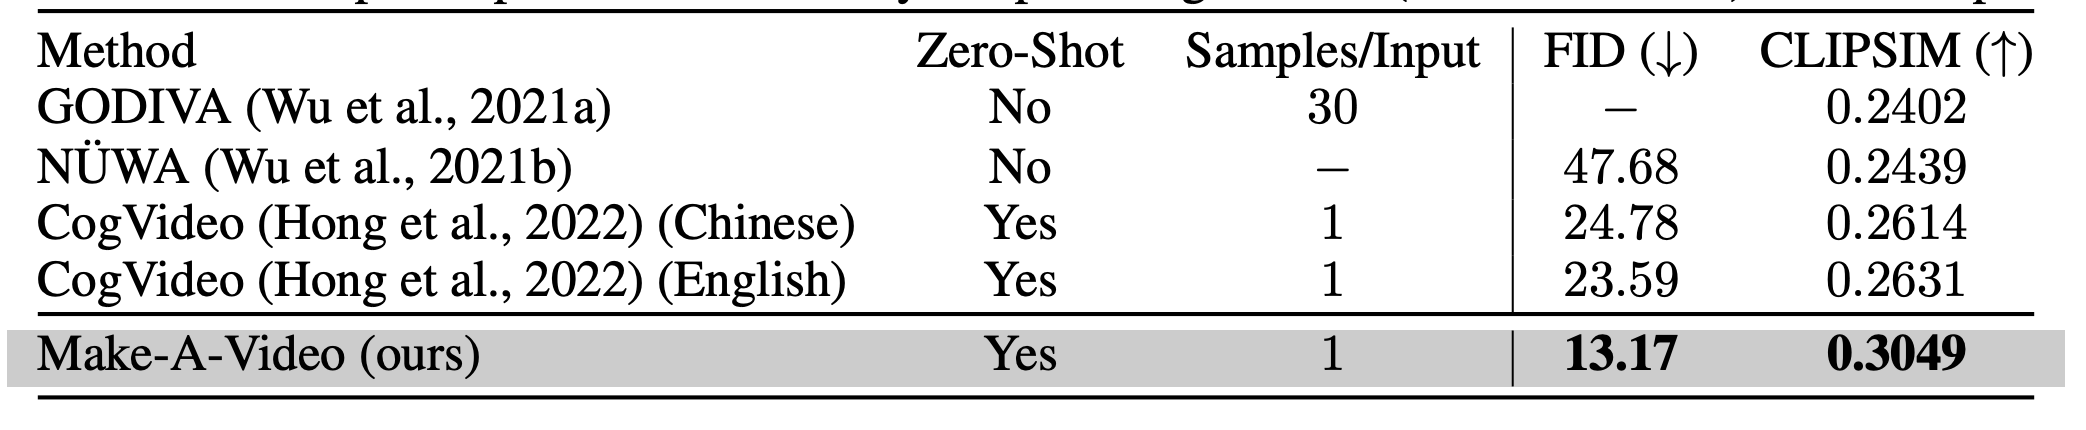
\includegraphics[width=1\textwidth]{images/make_a_video/zero_shot_eval.png}
    \caption{Make-a-Video significantly outperforms all state-of-the-art T2V generation models in zero-shot setting in both FID and CLIP-SIM score.}
    \label{fig:make_a_video_zeroshot_eval}
\end{figure}